\subsection{Discrete realization of the speed loop}
\label{sec:discrete}

Equation~\eqref{eq:motornum} is continuous. The feed computer is not. With a zero-order hold on the command and a sample $T_m=0.01$~s, the exact discretization of $\tau\dot\omega+\omega=u_{\omega}$ is a first-order difference
\begin{equation}
\omega_{n+1} = a\,\omega_n + (1-a)\,u_n, \qquad a = e^{-T_m/\tau}.
\label{eq:discplant}
\end{equation}
Substituting $\tau=0.18$~s gives $T_m/\tau=0.0556$ and $a=0.9460$. The one-step gain on the command is $1-a=0.0540$. A command that steps by 1~rad/s therefore moves the shaft by only 0.054~rad/s on the next sample, which is why the loop needs many samples to finish a bridge-induced ramp and why a 10~ms budget is comfortable for the arithmetic even though it is tight for a stall detector.

The proportional--integral law without the derivative, written backwards in time so that it can be coded as a recurrence, uses the summed error $s_n$ and the clamped increment
\begin{equation}
s_n =
\begin{cases}
s_{n-1}, & |e_n|>0.8~\text{rad/s or } u \text{ on its rail},\\
s_{n-1}+T_m e_n, & \text{otherwise},
\end{cases}
\label{eq:sum}
\end{equation}
and
\begin{equation}
u_n = \mathrm{sat}\big(K_p e_n + K_i s_n + K_d\,\delta_n\big),
\label{eq:usat}
\end{equation}
where $\delta_n$ is the filtered difference. The derivative filter is itself a discrete pole. A continuous pole at 40~Hz has time constant $1/(2\pi\cdot 40)\approx 4.0$~ms. Its exact sample coefficient at 10~ms is not the right object, because the difference is already a once-per-sample quantity. The implementation uses an exponential smoother on $\Delta e_n/T_m$,
\begin{equation}
\delta_n = \beta\,\delta_{n-1} + (1-\beta)\,\frac{e_n-e_{n-1}}{T_m}, \qquad \beta = e^{-T_m/\tau_d},
\label{eq:dfilt}
\end{equation}
with $\tau_d=4$~ms, so $\beta=e^{-2.5}=0.0821$. The filter is fast relative to the motor and slow relative to a single-sample encoder spike. An encoder that glitches by one count on a 4096-count wheel at 22~r/min produces a false $\Delta\omega$ of $2\pi/4096$ radians in 10~ms, which is 0.15~rad/s of false rate. Multiplied by $K_d=0.08$ that glitch is a 0.012~rad/s command bump, smaller than the tracking residual already budgeted in the estimation. The filter is what keeps a two-count glitch from becoming a command. This arithmetic is the sort of check that belongs in the feed computer's design review. It is not a result from a logic analyser.

Integral separation and the rail clamp interact. If the clamp freezes $s_n$ while the separation condition is also true, the sum is frozen once, not twice. The code path must be a single conditional. Two nested conditionals that both subtract the last addition will drift. The specification is Equation~\eqref{eq:sum}: one freeze flag, the logical or of the two reasons.

\subsection{A numerical fuzzy step}

The rule table is easier to trust after one sample is evaluated by hand. Take $e_n=0.30$~rad/s and $e_{n-1}=0.35$~rad/s, so the shaft is below the command and the error is shrinking. The scaled inputs of Equation~\eqref{eq:scalee} are
\begin{equation}
\tilde e = 0.30/0.6 = 0.50, \qquad \widetilde{\Delta e} = (0.30-0.35)/0.15 = -0.333.
\end{equation}
On the error partition of Figure~\ref{fig:member}, $\tilde e=0.50$ sits on the peak of the positive-small triangle, so $\mu_{\mathrm{PS}}(\tilde e)=1$. The positive-big trapezoid is 0 at 0.4 and 1 at 1.0, so
\begin{equation}
\mu_{\mathrm{PB}}(\tilde e) = (0.50-0.40)/(1.00-0.40) = 0.167.
\end{equation}
Zero, negative-small, and negative-big are 0 at this point. On the increment, $-0.333$ falls inside the negative-small triangle centred at $-0.5$ with support from $-0.9$ to $-0.1$. The left slope would be irrelevant. The right slope runs from membership 1 at $-0.5$ to 0 at $-0.1$, and $-0.333$ is $(0.5-0.333)/0.4=0.417$ of the way from the centre to the edge, so $\mu_{\mathrm{NS}}(\widetilde{\Delta e})=1-0.417=0.583$. The zero triangle has support $[-0.4,0.4]$ and peak 1 at 0, so at $-0.333$ its membership is $1-0.333/0.4=0.168$. Negative-big is the trapezoid that is 1 at $-1$ and 0 at $-0.4$. At $-0.333$ it is already 0.

Four rule conjunctions survive, using the minimum for ``and''. From Table~\ref{tab:fuzzy}, error positive-small and increment negative-small fires $\Delta K_p$ at label Z with strength $\min(1,0.583)=0.583$. Error positive-small and increment zero fires NS with strength $\min(1,0.168)=0.168$. Error positive-big and increment negative-small fires NS with strength $\min(0.167,0.583)=0.167$. Error positive-big and increment zero fires NS with strength $\min(0.167,0.168)=0.167$. The output labels are placed at Z$=0$ and NS$=-0.5$ on the increment universe. Aggregating by the maximum, the Z spike has height 0.583 and the NS spike has height $\max(0.168,0.167,0.167)=0.168$. A centroid of two spikes is
\begin{equation}
c = \frac{0.583\cdot 0 + 0.168\cdot(-0.5)}{0.583+0.168} = -0.112.
\end{equation}
Scaled into the proportional box $[-0.8,0.8]$, the increment is $\Delta K_p=-0.090$. The nominal $K_{p0}=2.4$ becomes $K_p=2.31$. The loop is close to the command and the error is already shrinking, so the scheduler slightly reduces proportional gain rather than kicking the shaft. A large growing error would have fired the PB corner of the table and moved $\Delta K_p$ the other way. The example is the ordinary sample, which is the sample the machine sees most often. A design that only behaves well on the linguistic corners and chatters in the middle is the design this calculation is meant to forbid.

The same sample's integral rules, which cut $K_i$ away from zero error, produce a small negative $\Delta K_i$ because $\tilde e$ is not inside the zero label. Derivative rules see an error and an increment of opposite signs, so they do not raise $K_d$. The net command correction relative to the nominal triple is a few percent. That is what ``bounded schedule'' means in a number rather than in a slogan \cite{mamdani1974,takagi1985}.

\subsection{Flight after release}
\label{sec:flight}

The spacing model in the estimation advances the tractor by $X_t/\sigma$ and then adds a random scatter. The scatter has a mechanical source that should be written down so a bench can look for it. A seed leaves the cell at angle $\psi$ below the horizontal with speed $r\omega$ relative to the housing, and the housing moves at $v$. In a frame fixed to the ground at the release instant the initial velocity is
\begin{equation}
\dot x(0) = v - r\omega\cos\psi, \qquad \dot y(0) = -r\omega\sin\psi,
\label{eq:v0}
\end{equation}
with $y$ positive upward and the tube entrance a distance $L_t$ below the release. For the nominal wheel, $r=0.09$~m and $\omega=2.30$~rad/s, so $r\omega=0.207$~m/s. At $\psi=70^\circ$, which is a release on the lower rear of the wheel, $\dot x(0)=v-0.071$~m/s and $\dot y(0)=-0.195$~m/s. The time to fall $L_t=0.40$~m under gravity, ignoring wall strikes, solves
\begin{equation}
L_t = -\dot y(0)\,t + \tfrac12 g t^2.
\label{eq:fall}
\end{equation}
The positive root is $t=0.306$~s when $\dot y(0)=-0.195$~m/s. During that time the tractor moves $vt$. The seed's own $\dot x$ is smaller than $v$ by 0.071~m/s, so the seed lands $0.071\cdot 0.306\approx 0.022$~m behind the point a kinematic model would predict. Two centimetres is 0.09$X_t$. It shifts the whole row. It does not by itself create a miss, because every seed is late by a similar amount when $\omega$ tracks $v$. It creates a miss when $\omega$ and $v$ stop matching, which is exactly the ground-drive slip case, and it creates a double-looking pair when one seed glances off the tube wall and the next does not.

The random term $\varsigma$ in Equation~\eqref{eq:sigma_scatter} is the wall-glance term. Its baseline $0.07X_t=17.5$~mm is the same order as the kinematic lag just computed. The coefficients on harshness and depth add the extra glances that a shaking tube and a bouncing shoe produce. The estimation does not integrate Equation~\eqref{eq:fall} seed by seed. It would be a better bench model and a worse real-time model. The factor computer has no business integrating projectile motion at 5~Hz. The derivation is here so that a disagreement of about two centimetres between a tube gate and a belt is not mistaken for a control failure.

Bounce at the furrow bottom adds a second delay that depth error changes. A seed that strikes a shoe set 10~mm high spends longer in the slot and can roll. The depth servo's job, inside this derivation, is to keep that second delay repeatable. The 1.2~mm residual used when the coordinator is on is a statement that the second delay is then almost common mode and disappears from the spacing differences. The 6.5~mm residual used otherwise is a statement that it does not.

\subsection{Response times of the two computers}

The periods in Table~\ref{tab:params} are not a schedule until each task's worst-case execution is set against them. The feed computer has one control task. At a 2~ms budget inside 10~ms its utilization is 0.20. A single task at that utilization cannot miss a deadline unless the budget is a lie. The stall rule, two missed periods, is then a watchdog on the lie: if the timer interrupt is late twice, the motor current is removed. The watchdog is a hardware timer that the control task must kick. A software counter inside the late task will not count.

The vision and factor computer has two periodic tasks on one processor. Vision needs up to 30~ms every 50~ms. The search needs up to 40~ms every 200~ms. If vision is released first and runs to its budget, the search can start 30~ms into a vision period. In the worst phasing, vision is released again before the search finishes. Preemptive priority is given to vision, so the search is suspended. The search's worst-case response is its own 40~ms plus the vision executions that can preempt it. In 40~ms of search time at most one vision job is released, adding 30~ms, so the response is at most 70~ms. The deadline is 200~ms. The margin is 130~ms, which is the quantity that absorbs a slow frame, a checksum retry, and the logger. This is a response-time bound for two periodic tasks with one preemption edge, not a general schedulability theorem. It is enough for this task set because there are only two tasks and the higher one does not preempt itself.

The bound fails if the vision budget is wrong. A frame that takes 80~ms blows the 50~ms period and steals the margin from the search. The fault rule already treats a late feature datagram as a hold on $B$. The additional requirement is that a frame which overruns is aborted at 30~ms and published as a miss, rather than allowed to complete late and then count as a success. Aborting a late frame is what keeps the 70~ms bound true. Completing it ``just this once'' is how the corn vision meter lost the 6~km/h case \cite{borja2021}.

\begin{figure}[htbp]
\centering
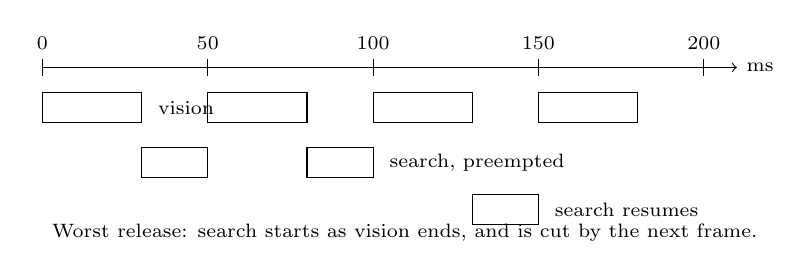
\begin{tikzpicture}[x=0.42mm,y=7mm,font=\scriptsize]
\draw[->] (0,3) -- (210,3) node[right] {ms};
\foreach \x/\lab in {0/0,50/50,100/100,150/150,200/200} {
  \draw (\x,2.85) -- (\x,3.15);
  \node[above] at (\x,3.15) {\lab};
}
\draw (0,2) rectangle (30,2.55);
\node[anchor=west] at (32,2.27) {vision};
\draw (50,2) rectangle (80,2.55);
\draw (100,2) rectangle (130,2.55);
\draw (150,2) rectangle (180,2.55);
\draw (30,1) rectangle (50,1.55);
\draw (80,1) rectangle (100,1.55);
\node[anchor=west] at (102,1.27) {search, preempted};
\draw (130,0.15) rectangle (150,0.7);
\node[anchor=west] at (152,0.42) {search resumes};
\node[anchor=west] at (0,0) {Worst release: search starts as vision ends, and is cut by the next frame.};
\end{tikzpicture}
\caption{Worst-case phasing used for the 70~ms response bound. Vision (top) preempts the factor search (bottom). The search still finishes inside the 200~ms deadline.}
\label{fig:schedule}
\end{figure}

\subsection{A slice of the cost grid}

The search is small enough that a slice of it can be printed. Table~\ref{tab:grid} evaluates Equation~\eqref{eq:cost} at the nominal red-oak diameter 20.5~mm with coefficient of variation 0.15, terrain frequency 6~Hz, slip 0.02, vision flag 0, and the predictor's terrain weight. The predictor does not use $\alpha_{\mathrm{iso}}=0.55$. It uses
\begin{equation}
f_{\mathrm{eff}} = \sqrt{0.35\,f_{\mathrm{dist}}^2 + f^2},
\label{eq:feffpred}
\end{equation}
which is a terrain coefficient $\sqrt{0.35}\approx 0.59$, slightly more pessimistic than the plant coefficient 0.55. The pessimism is intentional in the script that produces Chapter~\ref{ch:estimate}: the search plans for a worse mount than the plant applies. The difference is small. It is recorded here so that a reader who recomputes $f_{\mathrm{eff}}$ with 0.55 and does not match a grid point knows which constant moved.

\begin{table}[htbp]
\centering
\caption{Predicted cost $J$ for nominal red oak at a 6~Hz terrain frequency. Lower is better. Vacuum is in kPa and frequency in Hz.}
\label{tab:grid}
\begin{tabular}{@{}lrrrrr@{}}
\toprule
$f$ & $P=0$ & $P=1$ & $P=2$ & $P=3.5$ & $P=5$ \\
\midrule
3 & 3.052 & 3.157 & 3.267 & 3.443 & 3.631 \\
6 & 2.844 & 2.942 & 3.046 & 3.213 & 3.394 \\
9 & 2.171 & 2.255 & 2.346 & 2.494 & 2.657 \\
12 & 3.219 & 3.300 & 3.387 & 3.529 & 3.685 \\
\bottomrule
\end{tabular}
\end{table}

Every row prefers $P=0$. The vacuum term in Equation~\eqref{eq:zd} has no benefit at $\nu=0$ for this diameter, and the price 0.01 per kilopascal makes a useless vacuum strictly worse. The best printed point is 9~Hz and 0~kPa, with $J=2.171$. Twelve hertz is worse than 3~Hz because $f_{\mathrm{eff}}$ crosses the 10~Hz anchor: $\sqrt{0.35\cdot 36+144}=\sqrt{156.6}=12.5$~Hz. Nine hertz stays under it: $\sqrt{0.35\cdot 36+81}=9.59$~Hz. The Monte Carlo runs select this same corner for mild red oak, so the printed slice and the long runs agree on the nominal lot.

The harsh slice is a near-tie, and the thesis should say so rather than invent a wide margin. At $f_{\mathrm{dist}}=16$~Hz and $P=0$, the same nominal diameter gives $J(3)=3.052$ and $J(9)=3.052$, equal to three digits, with 9~Hz lower only in the fourth digit ($3.0521$ against $3.0522$). Four hertz and 8~Hz are worse, near 3.10 and 3.12. The agitation credit of sitting on $f^{\star}\approx 9.85$~Hz almost cancels the harshness of pushing $f_{\mathrm{eff}}$ to about 13~Hz. The recorded harsh-case run in Chapter~\ref{ch:estimate} selected 3~Hz because the search sees the sample mean of the drawn diameters, not the nominal 20.5~mm, and because a tie keeps the earlier grid point only when the later point is not strictly smaller. A sample mean a few tenths of a millimetre off nominal is enough to break a tie this close. The design consequence is practical. Under a 16~Hz disturbance the coordinator does not have a deep preference between a quiet command and the preferred agitation. Both beat the middle frequencies. A later bench that measures a true preference should replace the harshness coefficient before anyone treats 3~Hz as a unique optimum.

\subsection{Actuator lag and the slew limit}

The grid writes a step. The shaker and the regulator do not. Each is modelled, for the purpose of the slew numbers only, as a first-order lag
\begin{equation}
\tau_a \dot f_a + f_a = f, \qquad \tau_a \dot P_a + P_a = P,
\label{eq:lag}
\end{equation}
with $\tau_a\le 40$~ms so that a 2~Hz step is 95 percent complete in about 120~ms and a 1~kPa step likewise. The requirement stated in the stacking list was 150~ms. The lag model shows that the requirement is a time-constant requirement of about 40~ms, not a vague ``fast enough''. A shaker amplifier that is fast in current and slow in mechanical stroke will violate it even if the electrical specification looks fine. The stroke is the quantity in Equation~\eqref{eq:feff}.

The slew limit of 2~Hz per 200~ms step is 10~Hz per second, which a 40~ms lag can follow. The limit is therefore not hiding an actuator that cannot keep up. It is preventing the search from chattering between the 3~Hz and 9~Hz near-tie when the sample mean jitters. Without the slew, a mean that wanders by a tenth of a millimetre would bang the shaker between two equally good commands. With the slew, a change from 9~Hz to 3~Hz takes three periods, 0.6~s, which is about two or three cell events at 4.4~seeds/s. The seeds in between see an intermediate frequency. That intermediate is one of the middle frequencies the grid dislikes. The estimation does not simulate the slew. It applies the chosen command for the whole run, because each reported case has constant lot statistics and a constant disturbance. A bout in which the disturbance steps from 6~Hz to 16~Hz would pay a short transient the tables do not contain. The transient is bounded by 0.6~s of travel, about 0.7~m at 1.1~m/s, which is three target spacings. Three spacings are visible on a belt and invisible in a 4{,}000-event mean.

\subsection{Failure modes of the stack}

Table~\ref{tab:fmea} lists the failures that change a command, the detection that is actually implemented by the rules already stated, and the command that remains. A failure with no detection does not belong in a table that pretends to be an analysis. Those failures are listed as undetected on purpose.

\begin{table}[htbp]
\centering
\caption{Failures, the detection the design really has, and the command that remains.}
\label{tab:fmea}
\begin{tabular}{@{}p{32mm}p{38mm}p{62mm}@{}}
\toprule
Failure & Detection & Command that remains \\
\midrule
Late vision frame & Datagram age & Last $B$, then decay after 150~ms \\
Wrong scale factor in the camera & Not detected online & A biased $B$. Caught only by the disk calibration \\
Shaft encoder stop & Two missed periods & Motor current removed \\
Radar stuck at a high speed & Not detected online & $\omega^{\star}$ follows the stuck value. A separate timeout on acceleration would be a revision \\
Late factor search & Deadline at 200~ms & Previous $(f,P)$ \\
Search and plant disagree on $\alpha$ & Not a failure. The 0.35 weight is specified & Search is pessimistic relative to the plant \\
Vacuum transducer offset & Zero check at start only & A drifting offset reintroduces doubles. No in-bout zero \\
Depth potentiometer bias & Rail calibration only & A constant depth bias. Spacing scatter grows through $\varepsilon_h$ \\
Isolator collapse, $\alpha\to 1$ & Only if $f_{\mathrm{dist}}$ on the frame rises and the search reacts & The search sees the harsher frequency and moves $f$ \\
\bottomrule
\end{tabular}
\end{table}

Two rows deserve a longer remark because they are the ones a demonstration could hide. A stuck radar is worse than a dead radar. The dead case is specified: after 200~ms the command is held and then ramped to zero. A stuck high case looks like a healthy sensor that believes the tractor is moving. Seeds are metered onto a machine that is standing still, which piles wooden seeds in one spot. The design as written does not detect this. A revision that compares radar speed with the undriven-wheel encoder, and trips when they disagree by more than 15 percent for half a second, would close it. The revision is named here so that the gap is part of the design record rather than a surprise on the first stationary test.

A camera scale error is the other silent fault. The bridge index moves when the millimetre scale moves, because oversize in Equation~\eqref{eq:bridge} is a ratio of diameters. A scale that reads 10 percent high makes a 22~mm seed look like a 24~mm seed and under-calls the bridge. The disk calibration catches a scale error at service. Nothing catches it after the camera is knocked. A cheap in-bout check is the diameter implied by the tube-gate pulse width, which depends on seed size and not on the camera. The design logs the pulse width and does not compare it. The comparison is a consistent extension of the ``tube gate is a logger'' rule: the logger can audit the camera without entering the constraint. Putting the pulse width inside $B$ would couple a post-release sensor into a pre-release decision and would reintroduce the delay the cascade was built to avoid.

\subsection{Quantization, one cell period, and a two-step horizon}

The shaft encoder sets a floor under the fuzzy loop that the continuous model hides. A 4096-count encoder on the cell shaft has an angular quantum of $2\pi/4096=1.53\times 10^{-3}$~rad. At the 10~ms sample the corresponding speed quantum, if speed is a first difference, is $0.153$~rad/s. The nominal red-oak command is $2.30$~rad/s, so the quantum is 6.7 percent of the command if the difference is taken raw. That is coarser than the 0.012 tracking residual used in the estimation, and it would dominate the fuzzy input $\widetilde{\Delta e}$. The feed computer therefore does not differentiate adjacent samples alone. It fits speed over a window of $N_w=8$ samples, 80~ms, which divides the quantum by 8 and yields a speed quantum of about $0.019$~rad/s, just above the residual and just below the scale of $\Delta e$ that moves a membership from zero to small. Eighty milliseconds is 0.44 of the motor time constant, so the window adds lag of that order. The derivative filter of Equation~\eqref{eq:dfilt} and the window are redundant if both are naive. The specification is that the windowed speed is the feedback $\omega_n$, and the derivative filter runs on the tracking error of that already-windowed speed. A second difference of the raw counts is not computed.

The same 80~ms window is the right size relative to a cell. At $\omega=2.30$~rad/s a 12-cell wheel presents a new cell every $2\pi/(12\omega)=0.228$~s. The vision period, 50~ms, samples the throat about four times per cell. The motor period samples it about 23 times. The factor period, 200~ms, is almost one cell. A constraint that changes $\sigma$ therefore takes effect on the cell that is about to be filled, not on a cell that has already released. This timing is the reason the camera looks at the throat rather than at the tube. A tube gate 0.3~s later, from the flight calculation, reports a cell that the wheel has already left. Four vision samples per cell is also the budget inside which a single aborted frame, the 30~ms abort of the response-time argument, still leaves three frames. The bridge index is a vote across those frames through the one-pole filter of Equation~\eqref{eq:rhofilter}, whose 0.92 coefficient remembers roughly twelve frames. A one-frame lie decays. A real bridge, present for a third of a second, accumulates.

A two-step horizon is the natural objection to the one-step grid. Suppose the disturbance is known to step from 6~Hz to 16~Hz one period from now, and the command is 9~Hz. A two-step search could move toward 3~Hz on this period, arriving as the step arrives, whereas the one-step search waits to see 16~Hz and then slews. The value of that preview is the cost of three spacings of intermediate frequency, which the slew analysis already bounded at about 0.7~m of travel. Preview would save that 0.7~m. It would require a forecast of terrain frequency. The inertial unit's one-second Fourier window is a report of the past second, not a forecast of the next 200~ms. Using it as a forecast would be a model of the ground that this machine does not have. The one-step search is the controller that matches the sensor. A terrain map from a previous pass would justify a two-step, or a longer, horizon, and would be a different study, closer to the prescription maps of variable-rate cereal planting than to a single-row hardwood meter \cite{stafford2000,gebbers2010,liu2025review}.

The small-gain view of the constraint is similar in spirit. The map from $\sigma$ to the next bridge index is not known as a transfer function. What is known is a bound. The scale cannot fall by more than 0.22, and the occupancy filter cannot move by more than 0.08 of its input per vision sample. A scale cut therefore cannot chase its own tail inside one cell period: the wheel slows, the filter moves a small step toward the clear-throat target, and the next $\sigma$ is computed from a $B$ that has not yet fully forgotten the bridge. The loop can oscillate only if $B$ itself oscillates, which a real arch does not do at 20~Hz. The cap and the filter are the small-gain ingredients. They are not a computed gain margin. They are the structural reason a margin is plausible, and they are the knobs a bench would turn if the wheel hunted.

\subsection{Rates and power a builder can check with a stopwatch}

The kinematic numbers are simple enough to audit without the simulator, and they should be audited, because every later index is a fraction of them. At $v=1.10$~m/s and $X_t=0.25$~m the target is $\lambda^{\star}=4.40$~seeds/s, which is 264~seeds per minute and 15{,}840~seeds per hour. A 15~litre hopper holding acorns at a bulk density near 0.6~kg/L holds about 9~kg. Red-oak acorns near 4.6~g give roughly 2{,}000~seeds in a full hopper, which is $2000/4.40\approx 455$~s, or seven and a half minutes, of continuous metering. The hopper is a short-bout vessel on purpose. A refill warning at 15 percent mass fires with a little more than a minute left, which is enough to stop at the end of a pass and not enough to forget. Pin-oak seeds are lighter, so the same mass is more seeds and a longer bout. Bur oak is the opposite. The warning is on mass, not on a seed count, because the load cell does not know the species and the camera's count of the throat is not a count of the hopper.

The shaft speed that serves this rate, with twelve cells and a unit fill, is 22.0~r/min. A builder with a tachometer and an empty throat can command that speed and watch the encoder. The check does not need seeds. If the tachometer reads 22~r/min while the radar reads 1.10~m/s and the set spacing is 0.25~m, Equation~\eqref{eq:wstar2} is implemented. Seeds are what test the fill, not the arithmetic.

The energy proxy can be audited in the same spirit. The script accumulates $0.08\omega^2+0.012 f^2+0.02 P^2$ once per cell event. At the mild red-oak both-mode point, $\omega=2.30$~rad/s, $f=9$~Hz, and $P=0$, one event costs
\begin{equation}
0.08\cdot(2.30)^2 + 0.012\cdot 9^2 + 0 = 0.423 + 0.972 = 1.395,
\end{equation}
which matches the table entry 1.39. The shaker term is 70 percent of the proxy. At the harsh-case command $f=3$~Hz the shaker term falls to $0.012\cdot 3^{2}=0.108$, and the wheel term is unchanged, so the event cost falls near $0.53$, again the order of the harsh-case table. The proxy is not a wattmeter. It is a weighted sum that makes this comparison obvious: the camera and the fuzzy increments do not appear in it, and the shaker does. A builder who later measures current will not reproduce 1.39. A builder who finds that the shaker current is a small fraction of the wheel-motor current has discovered that the prices in $J$ were in the wrong ratio, and should raise the frequency price or lower the wheel weight before trusting the quiet-versus-loud tie. The functional form is the part worth keeping. The coefficients 0.08, 0.012, and 0.02 are placeholders until a current clamp replaces them.

Cell time and computer time meet in one inequality that is worth writing as a release check. A cell period is 0.228~s at the nominal rate. Inside that period the feed computer runs about 23 motor steps, the vision computer owes four frames, and the factor computer owes one search. The sums of the budgets are $23\times 2$~ms, $4\times 30$~ms, and 40~ms, which are 46~ms, 120~ms, and 40~ms. The vision budget sum, 120~ms, fits in 228~ms with 108~ms to spare, but only if the four frames do not stack. They do not stack if each frame is aborted at 30~ms, because $4\times 30=120<228$ and the frames are released 50~ms apart. The inequality $4\times 30~\mathrm{ms}<0.228~\mathrm{s}$ is the release check for the nominal speed. It fails at a shaft speed high enough that the cell period drops below 120~ms, which would be $\omega>2\pi/(12\cdot 0.120)=4.36$~rad/s, or about 42~r/min, corresponding to $v=2.08$~m/s at this spacing. The machine is not specified to run there. The inequality says why. It is the same lesson as the 6~km/h reversal on the corn meter, written as a speed limit that belongs to the vision budget rather than to the agronomy \cite{borja2021}.

\subsection{What an empty cell does to the count}

The rate audit above assumes every cell releases one seed. The indices exist because that assumption fails, and the failure has a counting form that is easy to misread on a display. Suppose that over $N$ cell passages the machine travels $N X_t/\sigma$ and releases $N_s$ singles and $N_d$ doubles, with the rest empty. The number of seeds is $N_s+2N_d$. The number of positive spacings is one less than the number of seeds, which for a long run is essentially $N_s+2N_d$. A double contributes a short spacing and also splits what would have been one interval into two, so it increases the spacing count. A miss contributes no spacing of its own. It lengthens a neighbour. The miss index is therefore not $100(N-N_s-N_d)/N$. That ratio is the empty-cell rate. The miss index is the fraction of observed spacings that exceed $1.5X_t$. If empties arrive in isolation, each empty lengthens one spacing from about $X_t$ to about $2X_t$ and the miss index is close to the empty-cell rate. If two empties arrive together, one spacing of about $3X_t$ replaces two empty cells in the count, and the miss index, which divides by the number of spacings rather than by the number of cells, moves differently from the empty-cell rate. The plantation looks worse. The percentage may rise or fall. The estimation's event model places isolated empties more often than bursts, because each event is drawn independently. A real arch lasts for several cells and would burst. The bridge constraint is the mechanism aimed at that burst: it slows the wheel while $B$ stays high, which is a run of cells rather than one draw. The independent-draw estimation therefore understates the value of the constraint on true arches and overstates the chance that a single slow cell is enough. That bias is a reason the both-mode gain on bur oak in Chapter~\ref{ch:estimate} should be read as a lower bound on what a persistent bridge would give the constraint to do, and as an upper bound on how tidy the resulting spacings would look. Independent draws make tidy tables. Arches make clumps. The controller is designed for the clumps. The table is computed from the draws. Both facts belong in the design record so that a belt test full of clumps is not scored as a refutation of a table that assumed none.

A twenty-cell strip makes the distinction numerical. Write E for an empty cell and S for a single, and ignore doubles. The release pattern
\[
\mathrm{S\,S\,E\,S\,S\,S\,E\,E\,S\,S\,S\,S\,E\,S\,S\,S\,S\,S\,E\,S}
\]
has five empties in twenty cells, an empty-cell rate of 25 percent. The spacings, in units of $X_t$ and dropping the final open end, are approximately
\[
1,\,2,\,1,\,1,\,3,\,1,\,1,\,1,\,2,\,1,\,1,\,1,\,1,\,2.
\]
Fourteen spacings follow. Four of them exceed $1.5$, so the miss index is $4/14\approx 29$ percent, against an empty-cell rate of 25 percent. The denominator shrank, because an empty cell does not create a spacing of its own, and the double empty became one spacing of 3 rather than two entries. A display that shows 25 percent skips from the tube gate, which counts empties, and a display that shows 29 percent miss index from a belt, which counts spacings, are both right. They are not the same statistic. The estimation reports the belt statistic, Equations~\eqref{eq:imult}--\eqref{eq:imiss}. The tube gate in the build reports the empty-cell rate through Equation~\eqref{eq:etahat}. An operator who treats them as one number will ``tune'' a controller that is already consistent. The design keeps them on different computers for that reason, not only for the deadline.

\subsection{What the extra analysis changes}

None of these calculations change the five modes of the estimation. They change what a disagreement with the estimation would mean. A two-centimetre bias is flight, not a bad gain. A tie between 3~Hz and 9~Hz is a flat cost, not a bug in the arg-minimum. A vision overrun that is allowed to finish is a broken response-time bound, not a mysterious rise in misses. The controllers remain the constraint of Equation~\eqref{eq:sigma} and the grid of Equation~\eqref{eq:cost}. The surrounding arithmetic is the part that makes those two equations implementable on the two computers of Section~\ref{sec:build} without confusing their faults with their tuning.
